\section{DevOps cycle and practices} DevOps concepts reflect in a set of practices during the DevOps delivery cycle. The cycle is visualised on a Figure 2.1. 

\begin{figure}[h]
\centering
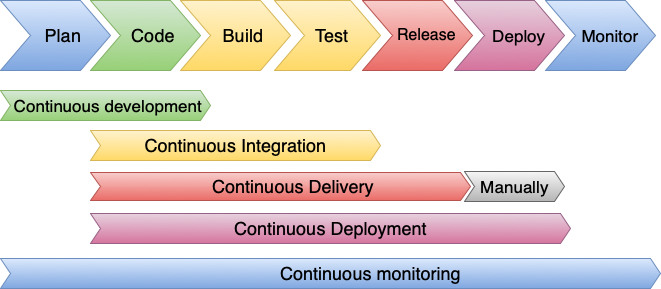
\includegraphics[scale=0.56]{../png/devops.png}
\caption{Devops cycle and practices}\label{picture:devops}
\end{figure}

\subsection{Continuous development} Continuous development is a practice composed of agile planning and coding. The goal of agile planning  is to divide big problems for smaller logical problems, estimate the complexity of created tasks and plan the amount of tasks for some short time period(sprint), usually it is from one to four weeks period. This method allows to get some large significant task done in a shorter time, because after its division developers can work on the subtasks simultaneously and it is more effortless for testing.

\subsection{Continuous integration (CI)} In order to avoid a problem with integration of large parts of code, Devops CI offers continuously pushing the code changes to the remote shared repository on the server. Every change pushed to the repository triggers a build and tests configured in a CI pipeline to make sure new changes did not affect already functioning functionalities and also does not contain new errors.

\subsection{Continuous delivery (CD)} Continuous delivery is an extension of continuous integration. After building and testing the code from the repository it automatically deploys releases to the testing environment and also prepares it to be deployed to the production. It requires human intervention to deploy a release to production. This is a safer version of fast and frequent deployment, in a case when the pipeline does not contain strong testing tools and application needs to be tested manually.

\subsection{Continuous deployment (CDE)} Coupled with continuous delivery, continuous deployment also deploys the release to the production. Using this practice no human intervention is required. Every change pushed to the main shared remote repository will be automatically deployed to production. The only obstacle for the deployment would be a failed build or test.

\subsection{Continuous monitoring (CM)} 

\subsection{Infrastructure as Code (IaC)}

\subsection{Containerization}




% \noindent Together with the constant improvement concept, automation is represented by a set of practices.


% Automation is a key element of a CI/CD pipeline, more about CI/CD in section 2.3.



% implications.. why we should or should not adopt it... what should we start with... CI, CD - yes ... others - think and discuss!

% https://www.techtarget.com/searchitoperations/tip/Carefully-weigh-these-DevOps-pros-and-cons

% https://www.orientsoftware.com/blog/advantages-and-disadvantages-of-devops/